\section{Character-based Word-Embeddings}
\label{sec:c2w}

\subsection{Introduction}

% Feeding character sequences to bidirectional LSTMs

The Compositional Characters to Word (C2W) Model is a new way to generate word embeddings 
presented by~\cite{DBLP:journals/corr/LingLMAADBT15}.
The input of the C2W model is a single word $w$, and we want to get a $d$-dimensional vector by which to represent $w$.
The basic idea is to let two LSTMs 'read' the word, by feeding them the word as a sequence of characters forwards and backwards.
The two resulting output states are then combined into the vector representation of the word.
%A commonly previously used approach is to treat the word embeddings as optimizable parameters
%in some kind of language model. 

The previous approach to build a NNLM as presented in~\ref{subsec:cslm} has some drawbacks which the C2W seeks to avoid:
\begin{enumerate}
  \item Each word embedding vector is independent. A word lookup table cannot generate representations for an unknown word, 
        even though it might have seen similar words before.
        A model might capture the linear correspondence of \textit{cat} and \textit{apple} compared to \textit{cats} and \textit{apples}, 
        but it doesn't capture that the added \textit{s} is responsible for this transformation. 
        It can't compute the same for a previously unseen plural word, even though it might know the singular version.
  \item For a large vocabulary it becomes impractical to actually store all word embeddings in a table.
\end{enumerate}
The C2W model avoids the first problem by breaking down words into their components. These components are then composed
back into the the representation of the word. There are previous efforts (\cite{Luong-etal:conll13:morpho}, \cite{DBLP:journals/corr/BothaB14}) 
which explore this idea, by breaking up words into their \textit{morphemes}. A morpheme is the smallest grammatical unit of a language 
e.g.\ "Unbreakable" comprises three morphemes: un-, -break-, and -able.
The downside of this approach is that you need a morphological analyzer to break down words. The C2W avoid this dependency by
breaking down words directly into characters.

\begin{wrapfigure}{r}{0.5\textwidth}
  \begin{center}
    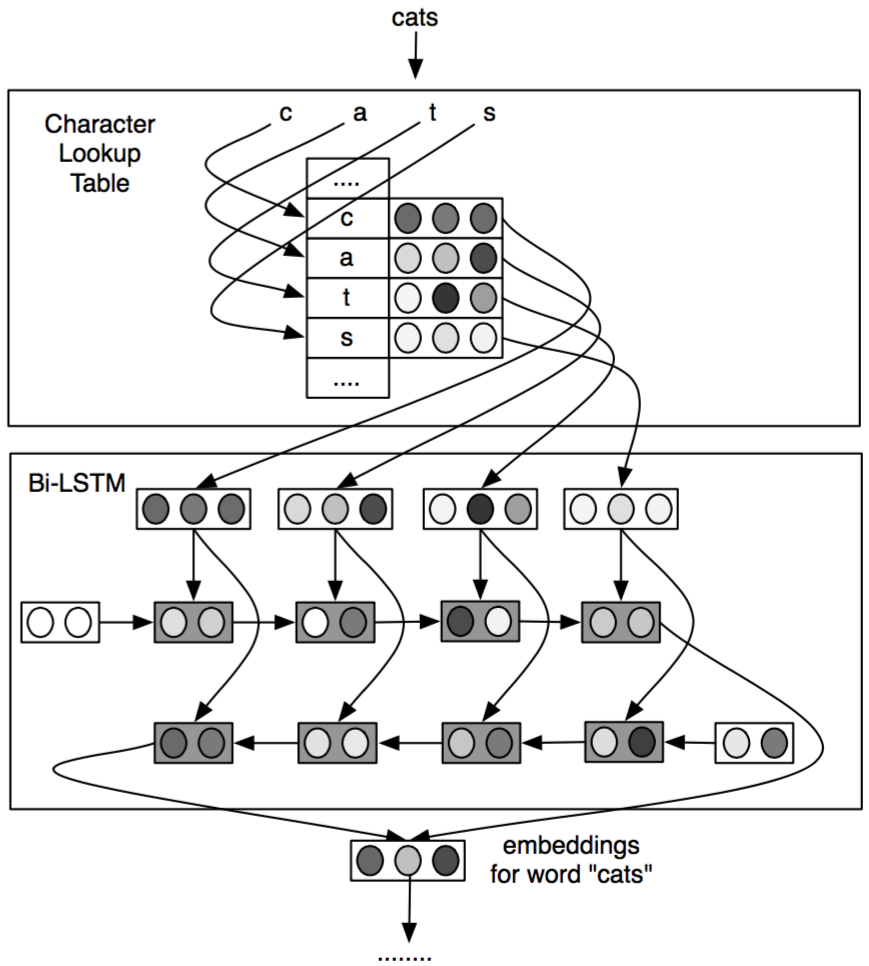
\includegraphics[width=0.5\textwidth]{./img/bi-lstm-emeddings}
  \end{center}
  \caption{Illustration of the lexical Composition Model (from~\cite{DBLP:journals/corr/LingLMAADBT15})}
\end{wrapfigure}

\subsection{Character Lookup Table}

The first processing steps involves a table of $d_C$ parameters for each character from a predefined character alphabet $C$.
Each word $w$ is decomposed into it's characters $c_1, \dots. c_m$.
Every input character gets transformed into a $d_C$-dimensional feature vector $e_{c_j}^C$ from this table.
These character feature vectors represent the properties of characters in the target language, for example consonants vs vowels.
The feacture vectors are stored in a projection layer $P_C \in \mathbb{R}^{d_C \times |C|}$ (Which is basically a lookup table for characters).
For each $c_j$ we can define the projection of our character as $e_{c_j}^C = P_C * 1_{c_j}$. In this equation the $1_{c_j} \in {0, 1}^{d_C}$ 
is a vector where all entries are zero except the entry corresponding to the index of the character$c_j$. 
The resulting sequence of character representations $e_{c_1}^C, \dots, e_{c_m}^C$ is then fed into the Bi-LSTM layer~\ref{subsec:bi-lstm}
in normal and reversed order.

\subsection{Bidirectional LSTM Layer}
\label{subsec:bi-lstm}

The second layer of the C2W model is a bidirectional LSTM layer~\cite{DBLP:journals/nn/GravesS05}. This consists of two LSTM blocks:
\begin{enumerate}
  \item The forward LSTM ($f$) which receives the sequence of character representations $e_{c_1}^C, \dots, e_{c_m}^C$
  \item The backward LSTM ($b$) which receives as input the reverse sequence $e_{c_m}^C, \dots, e_{c_1}^C$
\end{enumerate}
The two LSTM blocks yield the forward state sequence $s_{0}^f, \dots, s_{m}^f$ and backward state sequence $s_{m}^b, \dots, s_{0}^b$.
The reason for using a bidirectional LSTM is explained in a more detail in section~\ref{subsec:bidir-rnn}. A shortened explanation is 
that by supplying the network with the reversed input, it additionally gains access to previous context (previous characters).
 
The LSTM blocks are a little extended in comparison to the version introduced in section~\ref{subsec:lstm}.

The equations therefore look a little different:
% Given the input vectors x1,...,xm, a LSTM computes the state sequence h1, . . . , hm+1 by it- eratively applying the following updates:
\begin{equation}
\begin{aligned}  
  i_t &=\sigma(W_{ix} * x_t  + W_{ih} * h_{t-1} + W_{ic} * c_{t-1} + b_i) \\  
  f_t &=\sigma(W_{fx} * x_t  + W_{fh} * h_{t-1} + W_{fc} * c_{t-1} + b_f) \\
  o_t &=\sigma(W_{ox} * x_t  + W_{oh} * h_{t-1} + W_{oc} * c_t + b_o) \\  
  c_t &= f_t \odot c_{t-1} + i_t \odot \tanh(W_{cx} * x_t  + W_{ch} * h_{t-1} + b_c) \\ 
  h_t &= o_t \odot \tanh(c_t) 
\end{aligned}
\end{equation}
There are two seperate parameter sets for the LSTM block $\mathcal{W} = \{W_{ix},\dots,W_{ch},b_i,\dots,b_o\}$:
One for the forward LSTM ($\mathcal{W}^f$) and one for the backward ($\mathcal{W}^b$) LSTM.

\subsubsection{Bidirectional Recurrent Neural Networks}
\label{subsec:bidir-rnn}

The idea of a bidirectional recurrent neural network (BRNN) is to present every training sequence forwards and backwards to two separate
recurrent neural networks~\cite{IEEE:journals/singals/Schuster1997}.
Both networks are connected to the same output layer. This way the complete network has access to sequential information 
about all inputs before and after the current one.
This is illustrated in figure~\ref{fig:brnn-unfolded}, where the complete input is provided to the RNN twice (forwards and backwards).
\begin{figure}[H]
\begin{center}
  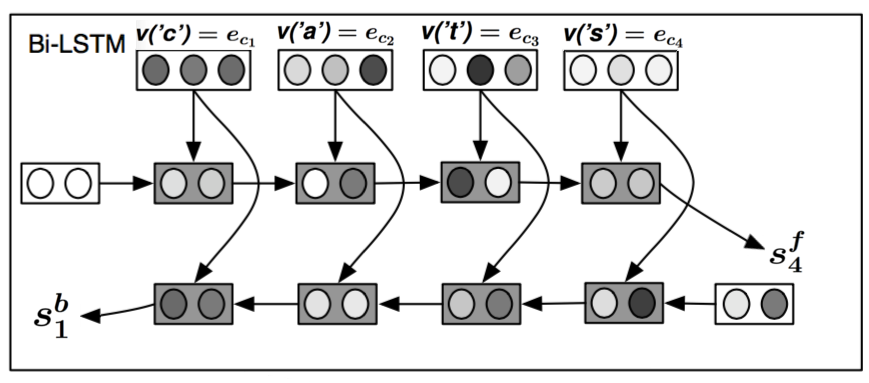
\includegraphics[width=\textwidth]{./img/brnn-unfolded}
  \caption{A generic BRNN unfolded for three timesteps (From~\cite{IEEE:journals/singals/Schuster1997}).}
  \label{fig:brnn-unfolded}
\end{center}
\end{figure}

The advantage of a BRNN is that there is no need to anymore manually specify how much context is 
used anymore (for example by having fixed-sized overlapping time-windows).
The net can decide to use as much or as little of the context as required. 
This can improve the results in sequence learning tasks, where the context can be previded in a "semi-online" fashion.
For example in online speech recognition an output after every sentences is fine~\cite{DBLP:journals/nn/GravesS05}. 



\subsection{Output-Layer}

Finally the last states of the forward sequence $s_{m}^f$ and the backwards sequence $s_{0}^b$
are linearly combined into the resulting word embedding $e_{w}^C$:
\[
  e_{w}^C = D^f s_{m}^f + D^b s_{0}^b + b_d
\]
The variables $D^f, D^b, b_d$ are the weights which determine how the states are combined.

Compared to using a lookup table computing $e_{w}^C$ is relatively expensive, but since the value only depends on
the word itself the value can be cached. This can be used for frequently occuring words to reduce the computational load.
At the same time not all words have to be cached, which reduces the amount of storage required for a large vocabulary.